\iffalse
Using section formula,
\begin{align}
         \myvec{-1\\6} &=\frac{{\myvec{-3\\10}+k\myvec{6\\-8}}}{1+k}\\
	 \implies 7k\myvec{1 \\ -2} &= 2\myvec{1 \\ -2}
	 \\
	 \text{or, } k &= \frac{2}{7}.
\end{align}
\fi
In 
			\eqref{eq:section_formula-k}, substituting
			\begin{align}
				\vec{B} &= \myvec{-3\\10}, \vec{C} = \myvec{6\\-8}, \vec{D} = \myvec{-1\\6},
				\\
				k &= \frac{\myvec{-2 & 4}\myvec{-7 \\ 14}}{\norm{\myvec{-7 \\ 14}}^2} = \frac{2}{7}
			\end{align}
\iffalse
See \figref{fig:10/7/2/4Fig1}.
\begin{figure}[H]
 \begin{center}
  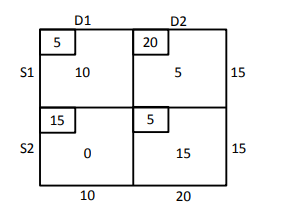
\includegraphics[width=0.75\columnwidth]{chapters/10/7/2/4/figs/fig.png}
 \end{center}
\caption{}
\label{fig:10/7/2/4Fig1}
\end{figure}
\fi
